\documentclass[12pt,a4paper]{article}

\usepackage[T1]{fontenc}
\usepackage[utf8]{inputenc}
\usepackage[margin=1in]{geometry}
\usepackage{amsmath,amssymb}
\usepackage{booktabs}
\usepackage{graphicx}
\usepackage{float}
\usepackage{placeins}
\usepackage{tabularx}
\usepackage{array}
\usepackage[expansion=false]{microtype}
\usepackage{natbib}
\usepackage[hidelinks]{hyperref}
\usepackage{url}

\title{Commodity Tail Dependence and Exchange-Rate Risk in Ghana:\\Copula Adequacy, Stress Tests, and Calendar Robustness}
\author{Jonathan Anthonio Nii Pedro Nelson\\Kwame Nkrumah University of Science and Technology (KNUST), Kumasi, Ghana\\\href{mailto:jonathannelson707@gmail.com}{jonathannelson707@gmail.com}\\ORCID: \href{https://orcid.org/0009-0006-9393-6237}{0009-0006-9393-6237}}
\date{Version 1 --- 6 October 2026}

\begin{document}
\maketitle

\begin{center}
\fbox{\parbox{0.88\textwidth}{\centering\textbf{Preprint --- not peer reviewed.}\\This manuscript is being circulated as a working paper prior to journal peer review.}}
\end{center}

\noindent\textbf{Short title:} Commodity Tail Dependence and Calendar Robustness

\begin{abstract}
This study examines commodity tail dependence and exchange-rate risk in Ghana using two co-equal calendar constructions for cocoa, gold, Brent crude oil, WTI crude oil and the Ghanaian cedi over 2015--2026. The analysis combines explicit marginal-model adequacy gates, absolute goodness-of-fit testing for eight static bivariate copula families, finite-threshold lower- and upper-tail concentration, and moving-block-bootstrap stress comparisons corrected for multiple testing. Across combined COVID-19 plus 2024 stress, COVID-19 alone and 2024 alone, no stress--calm comparison survives either Bonferroni or Benjamini--Hochberg correction in either calendar panel. Gold--Brent, Gold--WTI and Brent--WTI reject all eight tested static copula families under both calendar constructions. By contrast, Cocoa--Gold, Cocoa--Brent and Cocoa--WTI are calendar-sensitive, with complete rejection under business-day alignment but only partial rejection under common-observation alignment. All four commodity--cedi pairs reject none of the eight families in either panel, but the cedi remains inadequately represented by the tested continuous marginal models, so those copula and extreme-value estimates are interpreted conditionally. The results show that observation calendars, absolute model adequacy and multiplicity control materially affect which international-finance dependence conclusions are defensible.
\end{abstract}

\noindent\textbf{Keywords:} tail dependence; copulas; commodity risk; exchange-rate risk; Ghana; calendar alignment; stress testing

\section{Introduction}
\label{sec:introduction}

Ghana's external sector is highly exposed to commodity markets. UN Trade and Development classifies an economy as commodity-dependent when commodities account for more than 60\% of merchandise exports, and its 2025 country profile reports that Ghana's three leading commodity exports represented 78.4\% of allocated product exports over 2021--2023. Bank of Ghana data also underline the continuing importance of cocoa, gold and crude oil: in 2025, exports of cocoa beans and products were about US\$4.0 billion, non-monetary gold about US\$21.0 billion, and crude oil about US\$2.6 billion \citep{unctad2025,bog2025}. These exposures make the interaction between international commodity prices and the Ghanaian cedi relevant for financial risk measurement, portfolio decisions and the assessment of extreme market conditions.

The Ghana-specific literature already shows that commodity--currency relationships are nonlinear, asymmetric and horizon-dependent. \citet{zankawah2020} document spillover effects from crude oil prices to Ghana's exchange rate using multivariate GARCH models. \citet{archer2022} report asymmetric relationships between cocoa, gold, Brent crude oil and the exchange rate across quantiles, while \citet{boateng2022} document time-frequency variation between commodities and Ghanaian macroeconomic indicators. \citet{barson2023} find that commodity-return comovement varies across horizons and that the exchange rate plays an important role in those relationships. \citet{yeboah2025} similarly document nonlinear and asymmetric relationships between commodity prices and Ghanaian macroeconomic variables. More recent daily-frequency work links the cedi to global uncertainty and broader cross-market connectedness \citep{atipaga2025,woode2025}.

Copula methods themselves are not new in Ghana. \citet{mensah2020} estimate static and time-varying copulas for major foreign currencies against the cedi and report tail-dependent exchange-rate comovement. That result is an important novelty guardrail for the present paper. The contribution here is not the introduction of copulas to Ghanaian financial data. Instead, it is to ask whether commodity--cedi dependence, static copula adequacy and stress-period tail conclusions remain defensible when calendar construction, marginal adequacy and multiple testing are all made explicit.

International evidence likewise suggests that commodity--currency dependence varies with market state, commodity composition and model choice. Oil and exchange-rate comovement can strengthen after crises \citep{reboredo2012}, while time-varying tail dependence has been reported for major commodity currencies \citep{ignatieva2017}. Downside commodity tail risk is heterogeneous across currencies and commodities \citep{bondatti2022}, and dependence-switching approaches show that downside and upside spillovers can change across regimes \citep{ning2025}. Recent studies also document state-dependent return and volatility spillovers and changing commodity-currency relationships under political or crisis risk \citep{go2024,dodd2026}. Crisis-focused work finds stronger lower- and upper-tail contagion across commodity futures after the onset of COVID-19 \citep{qiao2023}. These results motivate direct analysis of extreme dependence, but they do not imply that every pair or every crisis window must exhibit stronger tail dependence.

Two methodological issues are especially important for the present setting. First, commodity futures and the cedi do not necessarily share the same observation dates or timing. Classical nonsynchronous-trading research shows that mismatched observations can distort return moments, correlations and cross-market dependence \citep{scholes1977,lo1990,martens2001,schotman2006}. More recent evidence also shows that synchronization choices can affect volatility-spillover inference during stressed periods \citep{dimitriou2025}. Calendar construction is therefore part of the statistical specification rather than a neutral data-cleaning step.

Second, relative model selection does not establish absolute adequacy. A lowest-AIC copula can still be misspecified, and misspecified marginal distributions can propagate error into copula and downstream risk estimates \citep{fantazzini2009}. Copula goodness-of-fit research therefore emphasizes resampling-based absolute tests under estimated parameters \citep{dobric2007,genestremillard2008,genest2009}. This distinction matters especially for the cedi, whose daily return distribution contains many exact zeros and whose selected continuous marginal specification does not pass the same probability-integral-transform adequacy gate as the commodity margins.

Tail inference raises a third issue. Finite-sample estimates of extreme dependence can be sensitive to the estimator, threshold and time variation \citep{frahm2005,supper2020}. The present study therefore reports empirical lower- and upper-tail concentration at prespecified finite thresholds rather than labelling these quantities asymptotic tail-dependence coefficients. Stress-period inference is conducted with a moving-block bootstrap, and multiplicity is controlled within each 60-test family using both Bonferroni and Benjamini--Hochberg procedures. This prevents isolated nominal p-values from being promoted to robust discoveries simply because many pair, threshold and tail combinations are examined.

Against this background, the paper uses two co-equal constructions of the same daily-source data for cocoa, gold, Brent crude oil, West Texas Intermediate (WTI) crude oil and the Ghanaian cedi over 2015--2026. Panel A imposes a business-day calendar with forward filling capped at three business days before returns are computed. Panel B uses only consecutive dates on which all five source series have actual observations and therefore contains no forward-filled return observations. Neither panel is designated as the primary or corrected dataset. A conclusion is described as calendar-robust when it survives both constructions and calendar-sensitive when its inferential classification changes.

The paper makes three contributions. First, it evaluates eight static bivariate copula families with an absolute Rosenblatt-transform Cram\'{e}r--von Mises goodness-of-fit procedure and parametric bootstrap rather than equating relative fit with correctness. Second, it compares empirical lower- and upper-tail concentration across calm periods and prespecified COVID-19 and 2024 stress windows using a moving-block bootstrap with family-level multiplicity control. Third, it treats the cedi's zero-heavy daily return distribution and marginal-model inadequacy explicitly, so commodity--cedi copula and extreme-value quantities are reported as conditional diagnostics rather than model-free structural parameters.

The analysis addresses three questions. First, do finite-threshold lower- and upper-tail concentration measures differ between calm and stress periods after multiplicity correction, and are the conclusions stable across calendar constructions? Second, can any of eight tested static bivariate copula families adequately represent the ten Ghana-relevant commodity and exchange-rate pairs, and which adequacy conclusions are calendar-robust? Third, how sensitive are cedi-related dependence and extreme-value diagnostics to the cedi's zero-heavy distribution, marginal-model inadequacy and calendar construction? The broader objective is to identify which international-finance dependence conclusions remain defensible after consequential data-construction and model-specification choices are made explicit.

\section{Data and Methods}
\label{sec:data_methods}

\subsection{Data and calendar construction}

The analysis combines daily-source-frequency prices for cocoa, gold, Brent crude oil and WTI crude oil from Yahoo Finance with the Ghanaian cedi exchange rate from the Bank of Ghana. Returns begin in January 2015. The cedi is signed so that positive returns denote appreciation and negative returns denote depreciation.

Two co-equal calendar constructions are retained. Panel A imposes a business-day calendar, carries missing prices forward for at most three business days, and then computes log returns. It contains 3,008 returns from 5 January 2015 to 15 July 2026. Panel B restricts the data to dates on which all five series have actual observations and computes returns between consecutive common dates. It contains 2,774 returns from 5 January 2015 to 10 July 2026. Panel B intervals range from one to six calendar days, with a median of one day. The two constructions therefore make different compromises: Panel A preserves nominal business-day frequency but can create carried-price zero returns, whereas Panel B removes forward-filled returns but does not represent a fixed 24-hour horizon.

\begin{figure}[htbp]
\centering
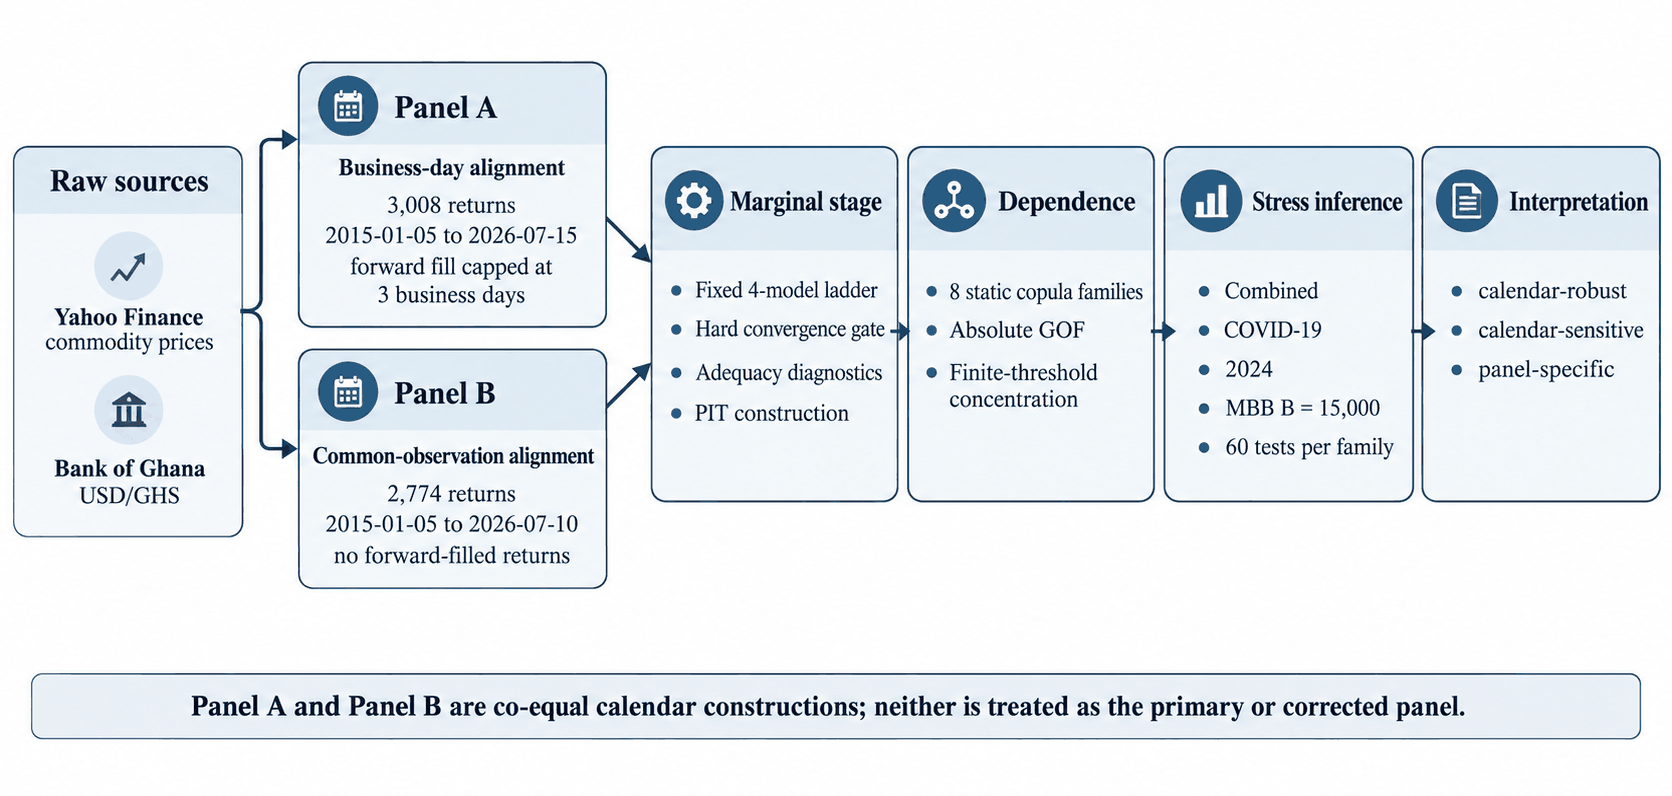
\includegraphics[width=0.98\linewidth]{figures/figure_01_calendar_workflow.png}
\caption{Data and calendar-construction workflow. Panel A uses business-day alignment with forward filling capped at three business days, whereas Panel B uses consecutive common actual-source dates without forward-filled returns.}
\label{fig:calendar-workflow}
\end{figure}

\begin{table}[htbp]
\centering
\caption{Calendar construction summary.}
\label{tab:calendar-summary}
\small
\begin{tabularx}{\textwidth}{lXX}
\toprule
\textbf{Feature} & \textbf{Panel A} & \textbf{Panel B} \\
\midrule
Alignment & Business-day grid & Common actual-source dates \\
Return observations & 3,008 & 2,774 \\
Return period & 5 Jan 2015--15 Jul 2026 & 5 Jan 2015--10 Jul 2026 \\
Missing-price rule & Forward fill, maximum 3 business days & No forward-filled return observations \\
Return interval & Nominal business-day & Previous common observation date \\
Exact Cedi zero-return share & 22.27\% & 16.51\% \\
Role in analysis & Co-equal specification & Co-equal specification \\
\bottomrule
\end{tabularx}
\end{table}

The WTI settlement of \(-37.630001\) on 20 April 2020 requires special treatment because a standard log return is undefined at a non-positive price. Panel A does not use that raw value directly in the log-return calculation and shifts the associated price movement to the next positive observation. Panel B drops the common interval affected by the non-positive value. The episode is retained as a documented data limitation rather than forced into an invalid logarithmic transformation.

Exact zero returns are materially more common in Panel A because of forward filling. For the cedi, however, the zero share remains high even in Panel B (16.51\%), indicating that the zero-heavy daily process is not solely an artifact of the business-day construction. This feature becomes important in the marginal-model diagnostics.

\subsection{Marginal filtering and pseudo-observations}

Each return series is filtered with a fixed four-model ladder: AR(1)-GJR-GARCH(1,1)-t, AR(2)-GJR-GARCH(1,1)-t, AR(1)-EGARCH(1,1)-t, and AR(1)-GJR-GARCH(1,1)-skew-t. A fit is eligible only if the optimizer converges and the likelihood, parameters, standardized residuals, conditional volatilities and probability-integral-transform (PIT) values are finite. Adequacy is assessed at the 5\% level using Ljung--Box tests on standardized residuals and squared standardized residuals (10 lags) and a Kolmogorov--Smirnov test of PIT values against Uniform(0,1). The first valid adequate model in the fixed ladder is selected. If none passes, the converged candidate with the lowest AIC is retained only as an inadequate reference model.

For a selected marginal model, standardized residuals are mapped through the fitted innovation distribution and then converted to rank-based pseudo-observations,
\[
u_t=\frac{\operatorname{rank}(\tilde u_t)}{n+1}.
\]
PIT values are clipped to \([10^{-6},1-10^{-6}]\) for numerical stability. A separate audit of the resulting Panel A cedi tie shows that restoring the underlying order changes no prespecified tail-set membership and produces only negligible changes in observed cedi-pair goodness-of-fit statistics.

\subsection{Copula specification and absolute goodness of fit}

With five series there are ten unordered pairs. Each pair is fitted with eight static bivariate copula families: Gaussian, Student-t, Clayton, Gumbel, Frank, Joe, survival Clayton and survival Gumbel. AIC is retained only as a relative-fit descriptor. Absolute adequacy is evaluated separately using a Rosenblatt-transform Cram\'{e}r--von Mises statistic with parametric bootstrap.

For fitted copula \(C_{\hat\theta}\), the Rosenblatt transformation is
\[
e_{1i}=u_i,\qquad e_{2i}=h_{\hat\theta}(v_i\mid u_i),
\]
and the transformed empirical distribution is compared with the product-uniform reference over a 50 by 50 grid. Each bootstrap replicate is simulated from the fitted family, re-ranked, re-estimated and retested. The Monte Carlo p-value is
\[
\hat p=\frac{1+\sum_{b=1}^{B} I\{S_n^{(b)}\ge S_n\}}{B+1}.
\]
All 80 pair-family cells are first evaluated with \(B=2000\); cells with initial \(0.03\le\hat p\le0.07\) are rerun with \(B=5000\). Rejection at 5\% is interpreted as evidence that the tested static family is inadequate under the implemented procedure. Non-rejection is not treated as proof that the family is the true model.

\subsection{Finite-threshold tail concentration and stress inference}

For pseudo-observations \((u_i,v_i)\), lower- and upper-tail concentration are measured at \(q\in\{0.025,0.05,0.10\}\):
\[
\hat\lambda_L(q)=\frac{1}{nq}\sum_{i=1}^{n}I(u_i\le q,v_i\le q),\qquad
\hat\lambda_U(q)=\frac{1}{nq}\sum_{i=1}^{n}I(u_i\ge 1-q,v_i\ge 1-q).
\]
These are finite-threshold concentration measures and are not described as asymptotic tail-dependence coefficients.

Stress--calm differences are evaluated under three prespecified stress definitions: COVID-19 (1 March--30 June 2020), calendar year 2024, and their union (Combined). For each definition, ten pairs, three thresholds and two tails produce 60 simultaneous tests. Inference uses a moving-block bootstrap with block length 20 and \(B=15{,}000\) replicates. Nominal p-values are reported descriptively, but confirmatory interpretation uses both Bonferroni family-wise-error control and Benjamini--Hochberg false-discovery-rate control within each 60-test family.

\subsection{Extreme-value and cedi diagnostics}

Extreme-value diagnostics use the loss transform of standardized residuals, \(L_t=-\hat z_t\), with a peaks-over-threshold generalized Pareto model above the empirical 90th percentile. The analysis records the GPD shape and scale parameters, 99\% VaR and expected shortfall, and threshold sensitivity. Because the cedi marginal fails the adequacy gate in both panels, cedi EVT estimates are interpreted only conditionally on the retained reference residual process.

Supplementary diagnostics examine cedi threshold sensitivity, alternative cedi treatments and the numerical effect of PIT clipping. These analyses are supporting checks rather than additional headline specifications.

\subsection{Use of generative artificial intelligence}

During manuscript preparation, the author used OpenAI's ChatGPT (GPT-5.6 Sol) to assist with code review, manuscript organization, language editing, consistency checking and preparation of publication materials. All analyses, numerical results, interpretations, references and final manuscript content were reviewed and verified by the author, who takes full responsibility for the work.

\section{Results}
\label{sec:results}

\subsection{Marginal adequacy}

The marginal stage produces a clear split between the commodity series and the cedi. Under both calendar constructions, each of the four commodities has at least one candidate that passes the stated residual, squared-residual and PIT adequacy gates. The cedi does not. In both panels the selected cedi specification is therefore an inadequate reference model rather than an adequate marginal representation. This distinction is carried into every cedi-related copula and EVT interpretation.

The calendar choice nevertheless changes the return process itself. Panel A contains materially more exact zero returns because carried prices create zero movements on some business days; the cedi zero share is 22.27\% in Panel A and 16.51\% in Panel B. The persistence of a high zero share in Panel B indicates that the cedi marginal problem cannot be attributed solely to forward filling.

\subsection{Finite-threshold tail concentration}

Figure~\ref{fig:tail-profiles} reports the empirical lower- and upper-tail concentration measures at \(q=0.025\), \(0.05\) and \(0.10\) for representative pairs in both panels. The profiles are treated as finite-threshold summaries, not as estimates of asymptotic tail-dependence coefficients. Their role is descriptive: the formal stress inference is based on the moving-block-bootstrap differences reported below.

\begin{figure}[htbp]
\centering
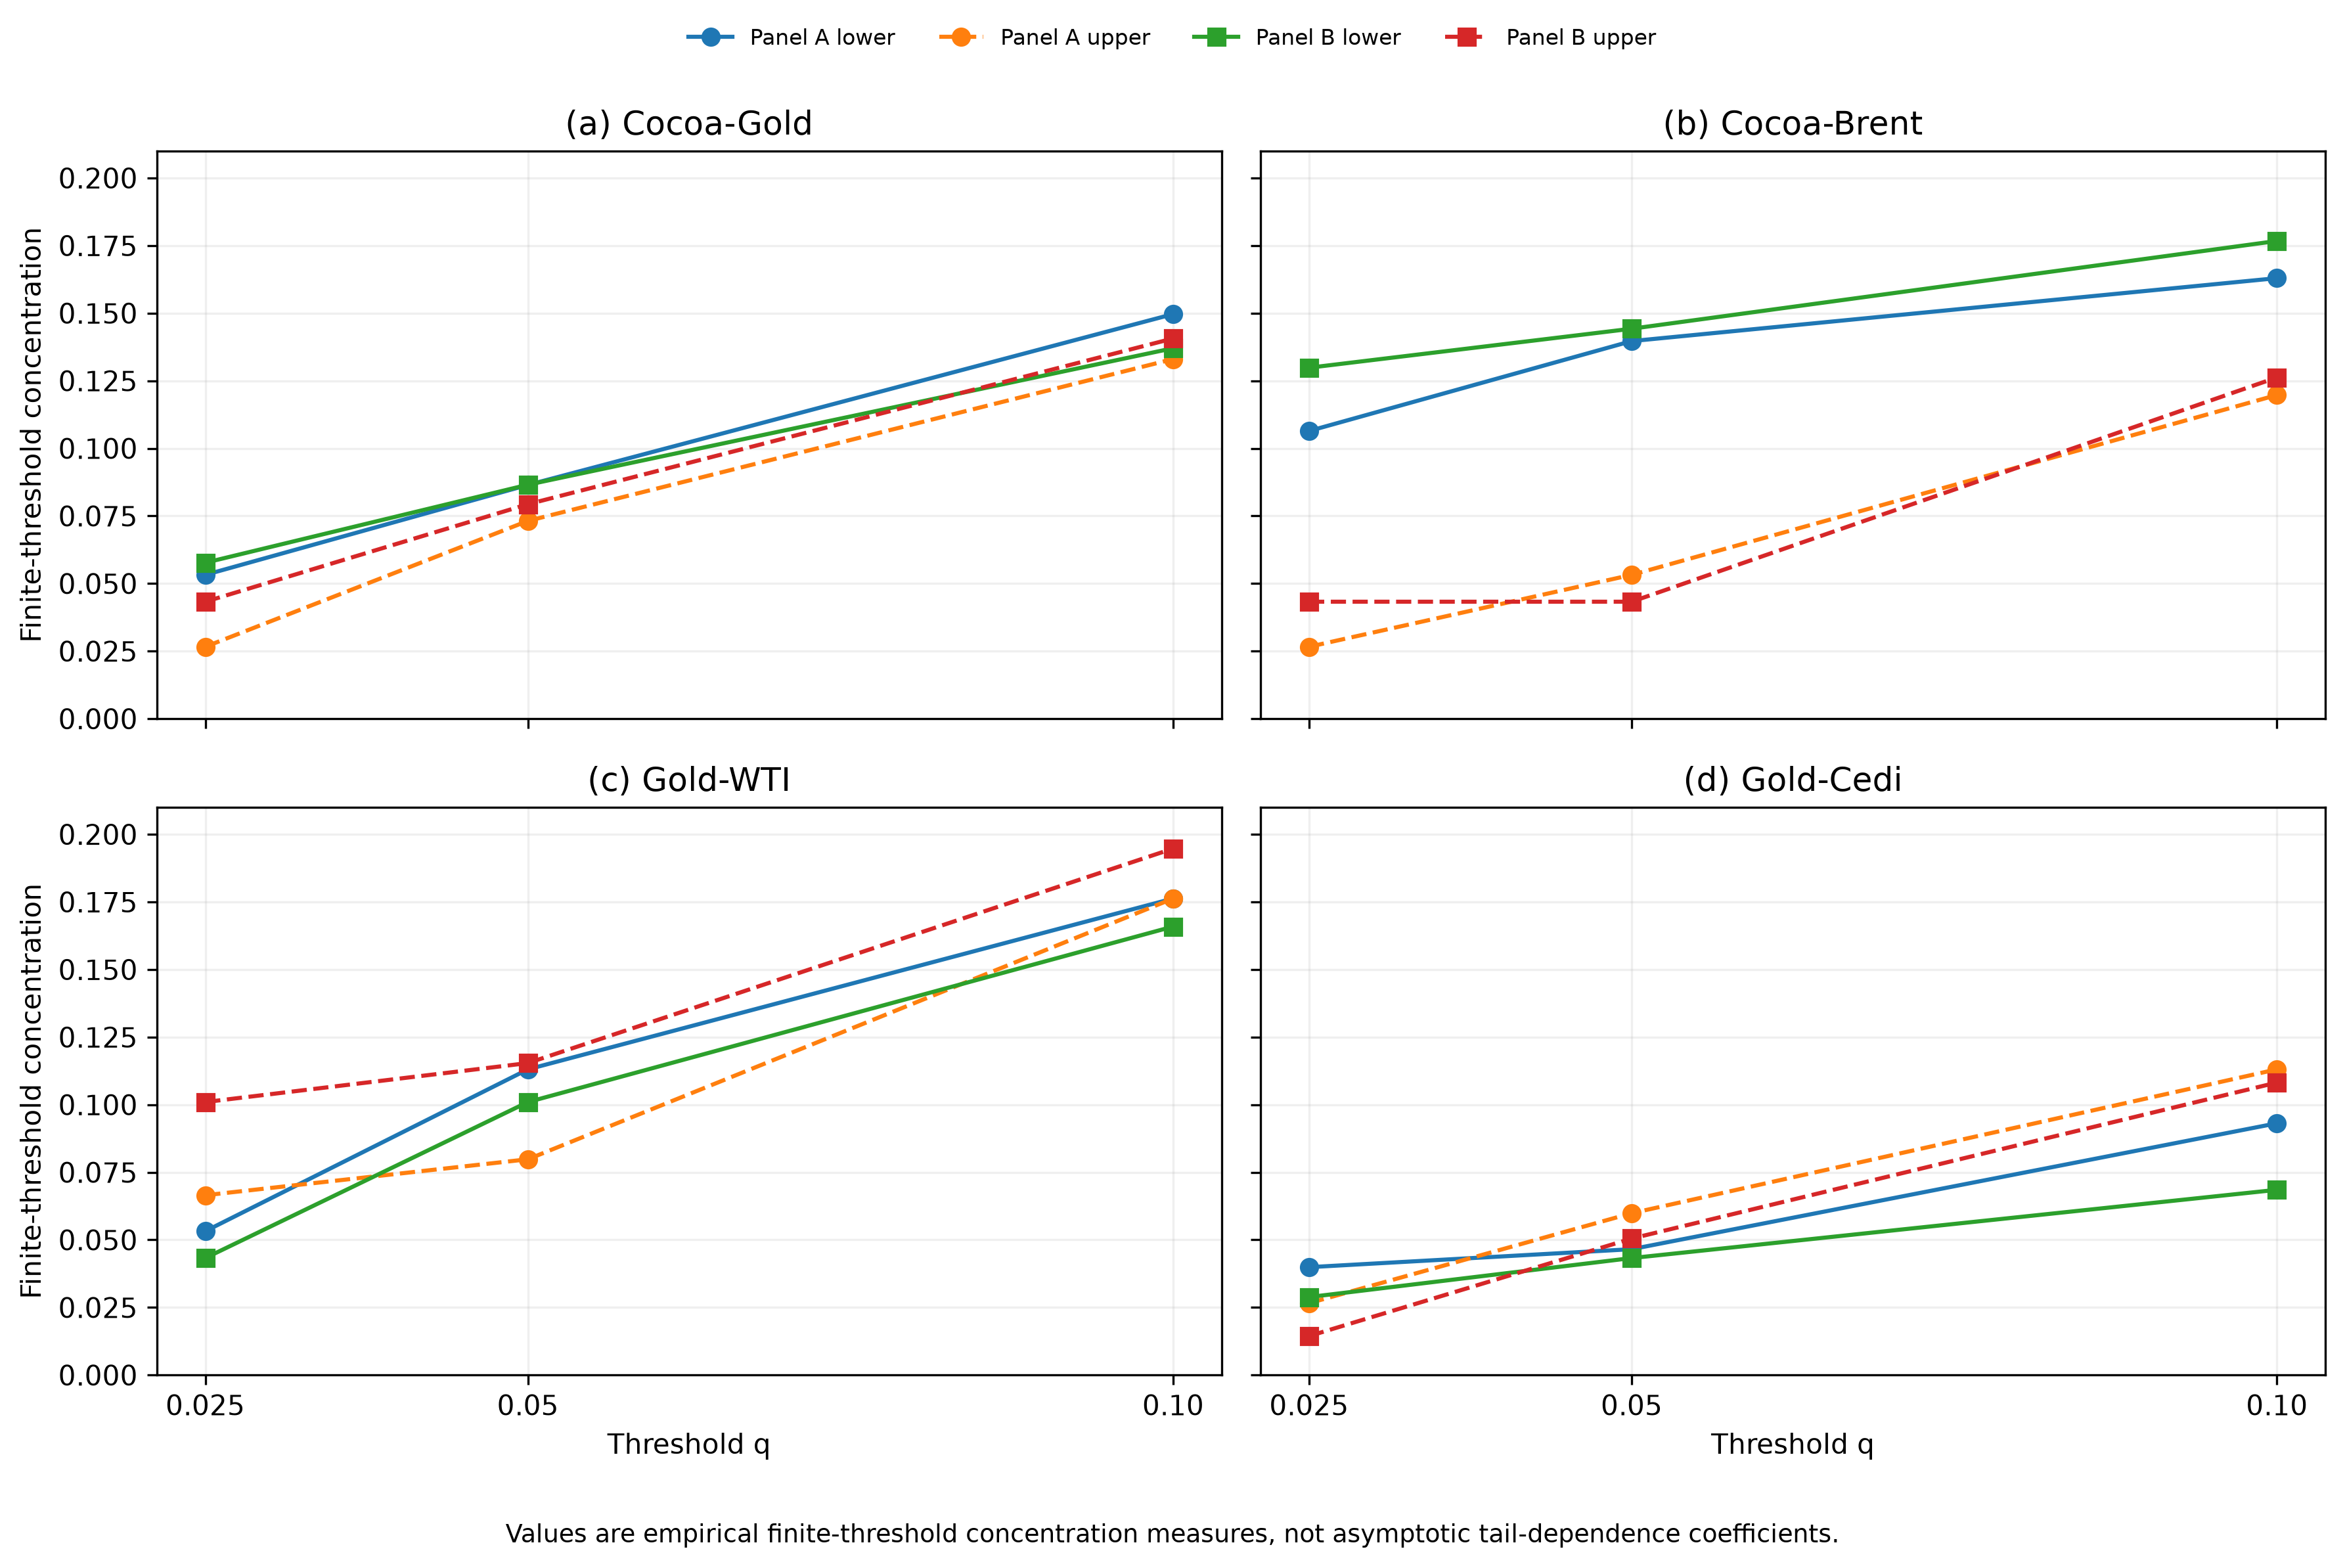
\includegraphics[width=0.98\linewidth]{figures/figure_02_tail_concentration_profiles.png}
\caption{Empirical finite-threshold lower- and upper-tail concentration profiles for selected pairs under the two calendar constructions.}
\label{fig:tail-profiles}
\end{figure}

\subsection{Static copula goodness of fit}

The strongest cross-panel distinction appears in the absolute copula goodness-of-fit results. Table~\ref{tab:gof} reports the number of rejected families, out of the eight tested, for each pair. Gold--Brent, Gold--WTI and Brent--WTI reject all eight families in both panels. These are calendar-robust rejections of the entire tested static family set.

The four commodity--cedi pairs show the opposite classification: none of the eight tested families is rejected for Cocoa--Cedi, Gold--Cedi, Brent--Cedi or WTI--Cedi in either panel. This is also calendar-robust, but it is interpreted cautiously because all four cells depend on the inadequate cedi marginal reference model. Non-rejection does not establish that the families are correct or equally plausible.

The three cocoa-related commodity pairs are calendar-sensitive. Cocoa--Gold, Cocoa--Brent and Cocoa--WTI reject all eight families in Panel A, whereas Panel B rejects only two of eight families for Cocoa--Gold and three of eight for Cocoa--Brent and Cocoa--WTI. Thus the adequacy conclusion for these pairs changes materially with the observation calendar even though the corresponding return series remain closely related across panels.

\begin{table}[htbp]
\centering
\caption{Static copula goodness-of-fit classifications across calendar constructions.}
\label{tab:gof}
\small
\begin{tabularx}{\textwidth}{lccX}
\toprule
\textbf{Pair} & \textbf{Panel A rejected} & \textbf{Panel B rejected} & \textbf{Classification} \\
\midrule
Cocoa--Gold & 8/8 & 2/8 & Calendar-sensitive \\
Cocoa--Brent & 8/8 & 3/8 & Calendar-sensitive \\
Cocoa--WTI & 8/8 & 3/8 & Calendar-sensitive \\
Cocoa--Cedi & 0/8 & 0/8 & Calendar-robust non-rejection \\
Gold--Brent & 8/8 & 8/8 & Calendar-robust rejection \\
Gold--WTI & 8/8 & 8/8 & Calendar-robust rejection \\
Gold--Cedi & 0/8 & 0/8 & Calendar-robust non-rejection \\
Brent--WTI & 8/8 & 8/8 & Calendar-robust rejection \\
Brent--Cedi & 0/8 & 0/8 & Calendar-robust non-rejection \\
WTI--Cedi & 0/8 & 0/8 & Calendar-robust non-rejection \\
\bottomrule
\end{tabularx}
\end{table}

\begin{figure}[htbp]
\centering
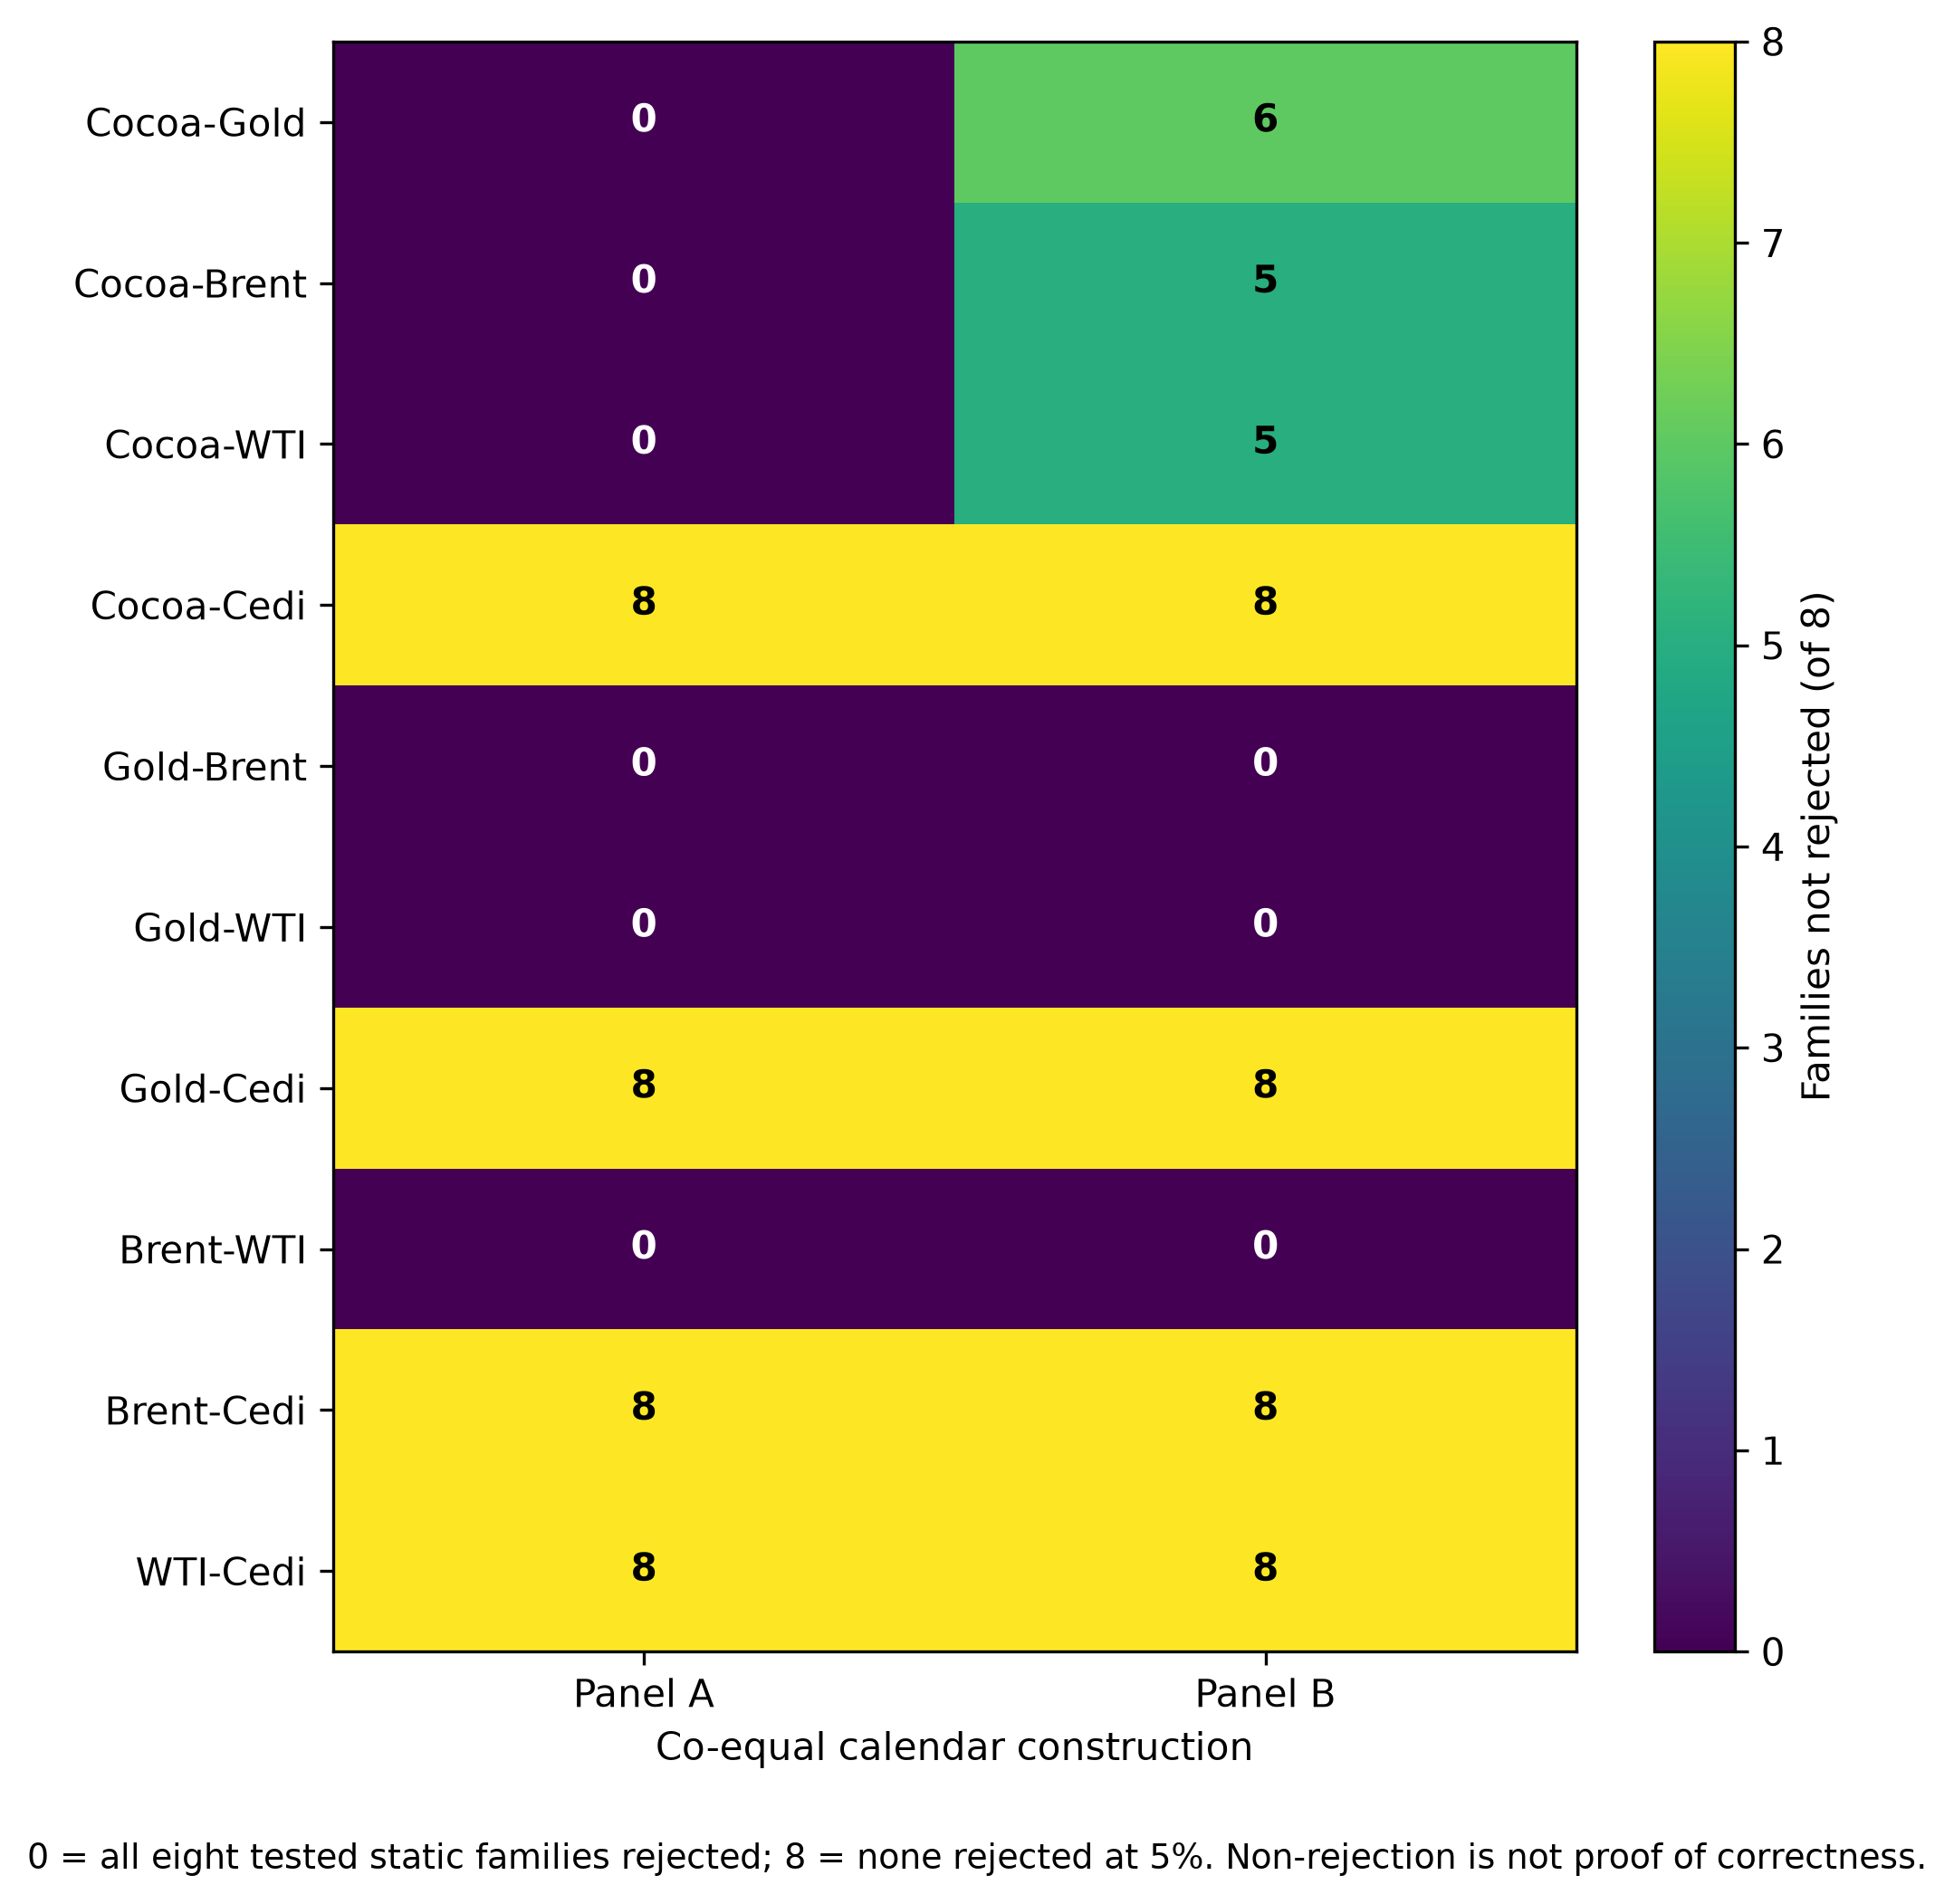
\includegraphics[width=0.96\linewidth]{figures/figure_03_copula_gof_heatmap.png}
\caption{Static copula goodness-of-fit across the two calendar constructions. Each cell reports the number of the eight tested families not rejected at the 5\% level.}
\label{fig:gof-heatmap}
\end{figure}

Figure~\ref{fig:gof-heatmap} displays the same pattern using the number of families not rejected. The contrast between the robust commodity-only rejection cells, the calendar-sensitive cocoa cells and the commodity--cedi non-rejection cells is visible without selecting a single ``best'' copula.

\subsection{Stress--calm inference}

Nominal stress evidence is present in both panels, but none survives multiplicity control. For the Combined stress definition, Panel A contains 6 nominal \(p<0.05\) cells and Panel B contains 5. COVID-19 alone produces 13 nominal findings in Panel A and 11 in Panel B. The 2024 definition produces 6 in Panel A and 7 in Panel B. After either Bonferroni or Benjamini--Hochberg adjustment, the number of discoveries is zero for every panel-by-stress family.

\begin{table}[htbp]
\centering
\caption{Nominal and multiplicity-controlled stress--calm test counts.}
\label{tab:stress}
\small
\begin{tabular}{lcccc}
\toprule
\textbf{Stress definition} & \textbf{A nominal} & \textbf{B nominal} & \textbf{Bonferroni A/B} & \textbf{BH A/B} \\
\midrule
Combined & 6/60 & 5/60 & 0/60; 0/60 & 0/60; 0/60 \\
COVID-19 & 13/60 & 11/60 & 0/60; 0/60 & 0/60; 0/60 \\
2024 & 6/60 & 7/60 & 0/60; 0/60 & 0/60; 0/60 \\
\bottomrule
\end{tabular}
\end{table}

\begin{figure}[htbp]
\centering
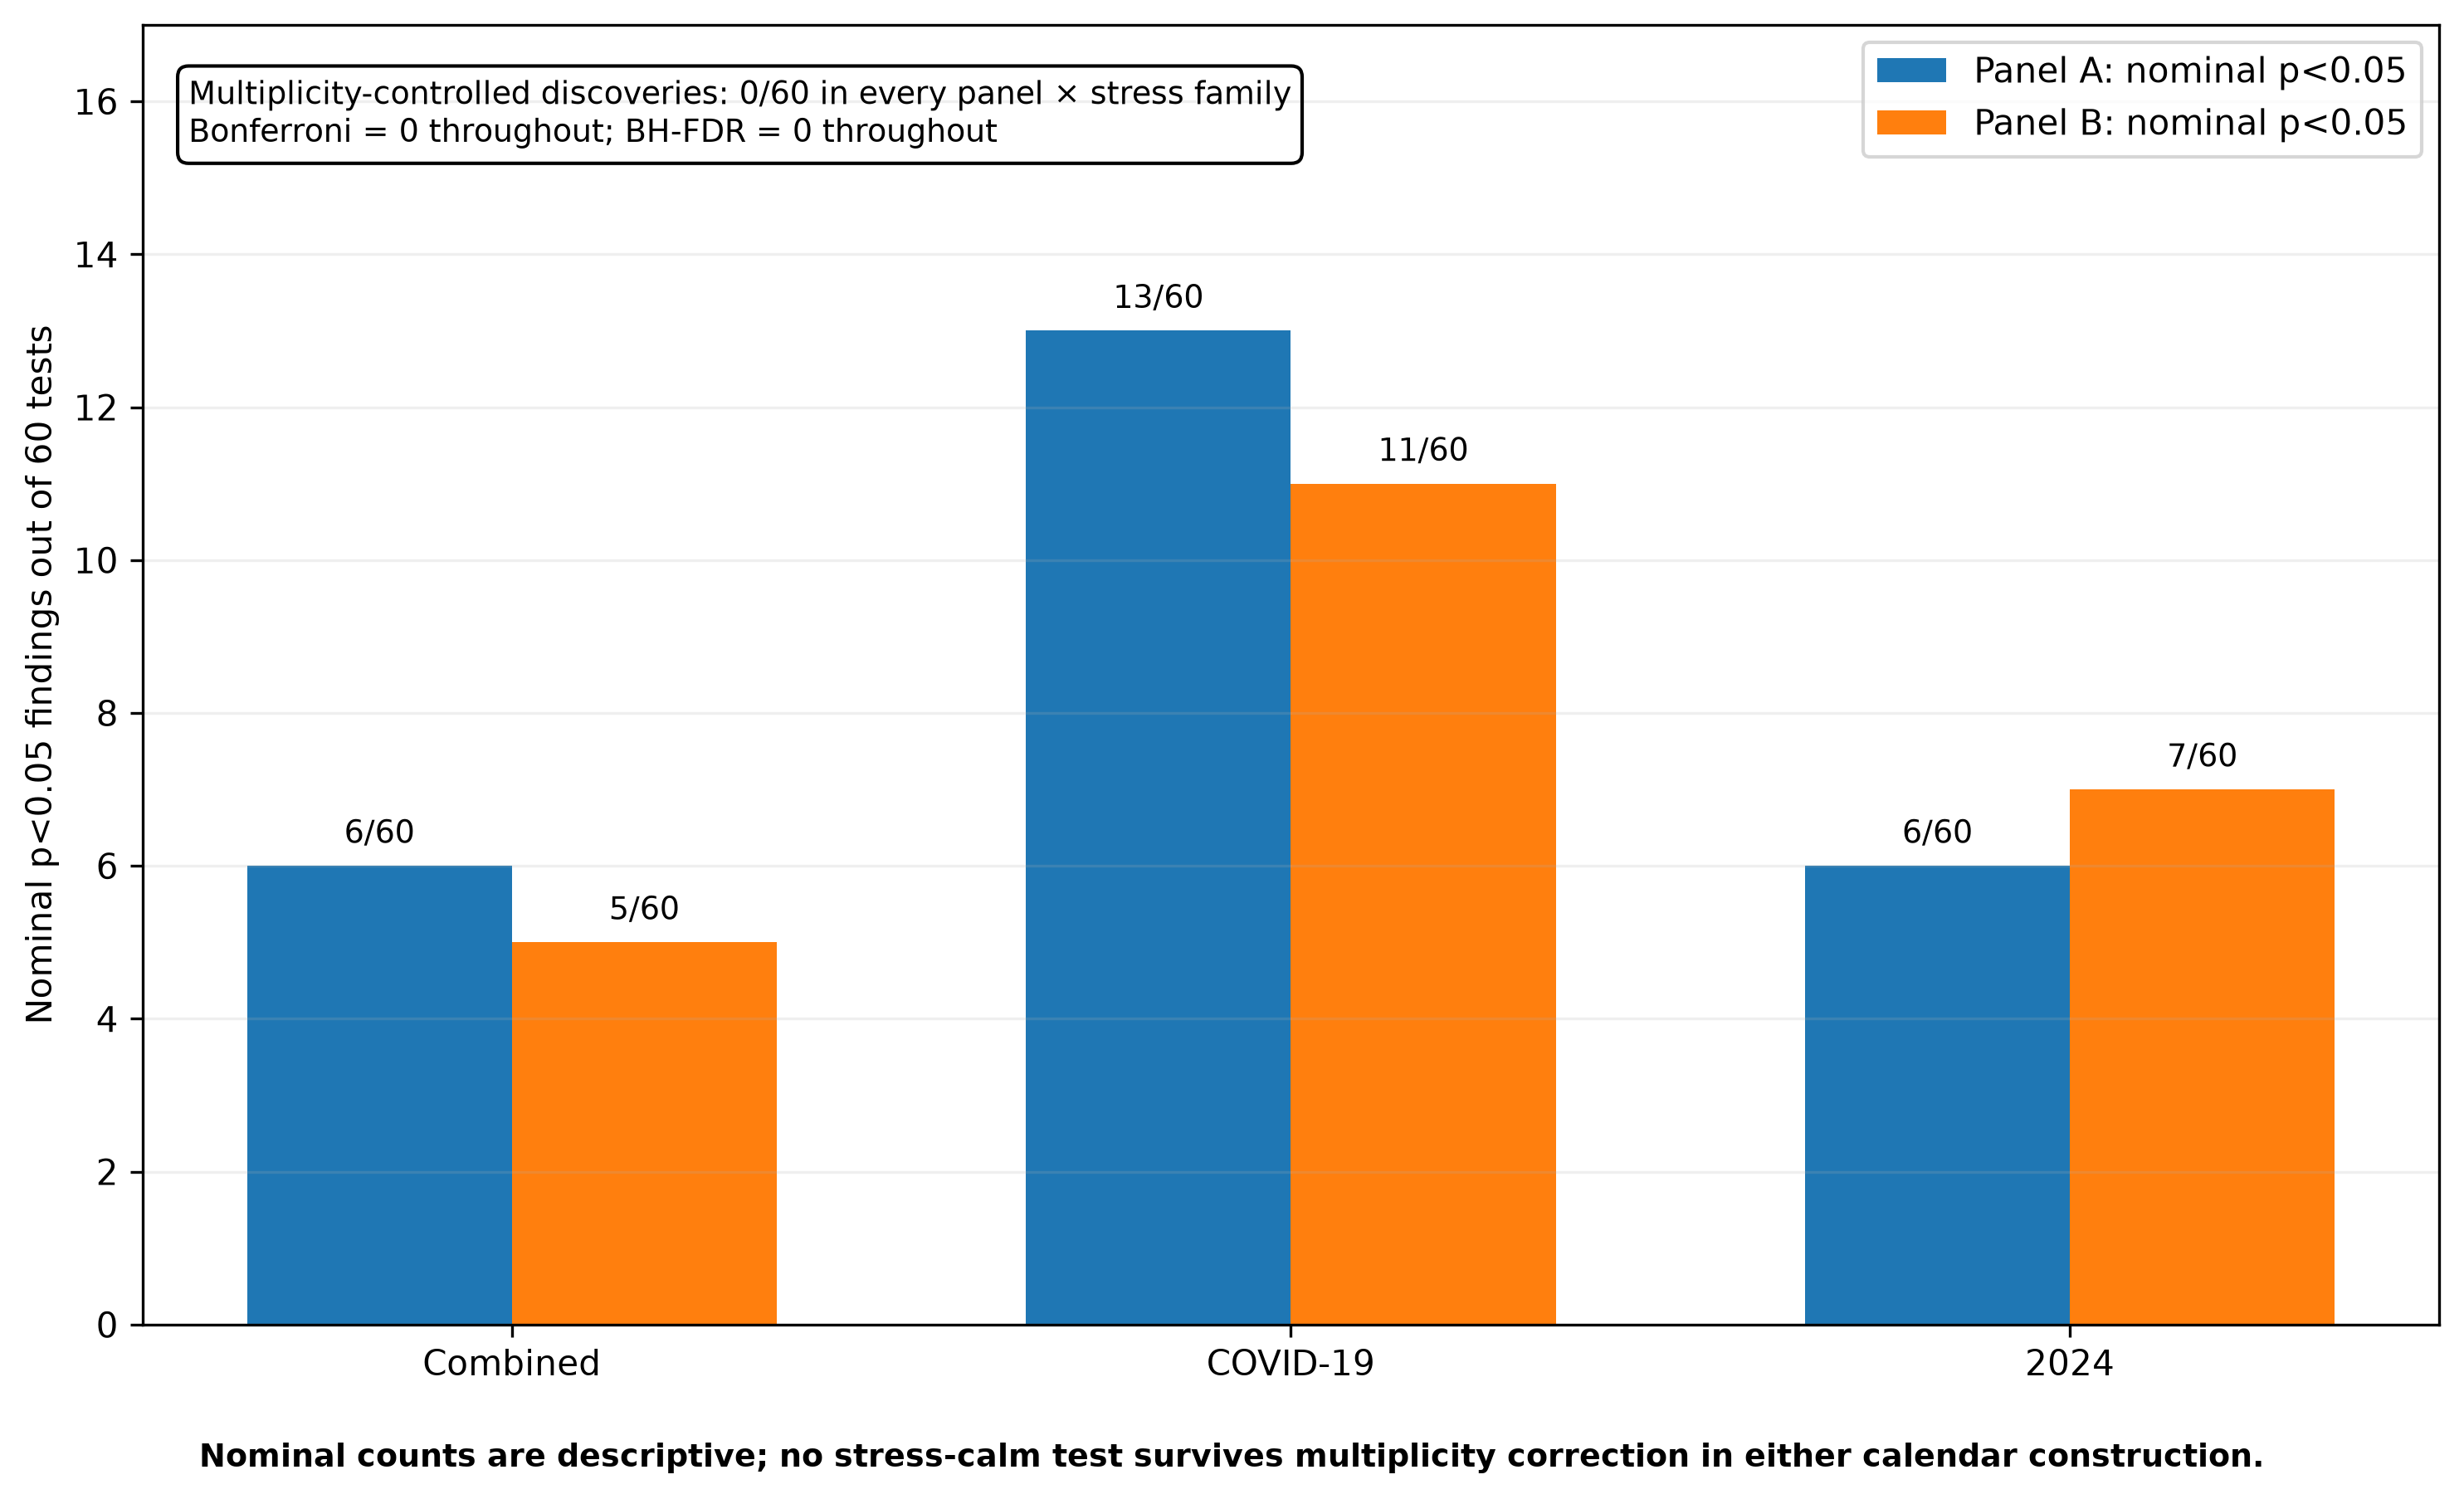
\includegraphics[width=0.92\linewidth]{figures/figure_04_stress_summary.png}
\caption{Nominal versus multiplicity-adjusted stress--calm findings across the two calendar constructions.}
\label{fig:stress-summary}
\end{figure}

The inferential conclusion is therefore calendar-robust: the tested stress-versus-calm differences do not provide corrected evidence strong enough to support an individual tail-concentration change under the prespecified thresholds, windows and bootstrap design. This statement is deliberately narrower than saying that market dependence was unchanged during COVID-19 or 2024.

\subsection{Cedi diagnostics}

The cedi remains the principal marginal-model limitation. The Panel B 90th-percentile POT/GPD fit gives approximately \(\hat\xi=0.693\) and \(\hat\beta=0.329\), with 99\% VaR of about 2.332 and 99\% expected shortfall of about 7.616 in standardized-residual units. Across threshold quantiles from 0.85 to 0.975, the fitted cedi shape parameter remains positive, approximately 0.63--0.79. These values are consistent with a heavy fitted loss tail under the retained reference process, but they are not treated as a model-free structural tail index because the cedi margin fails the PIT adequacy gate.

Supplementary diagnostics reinforce that caution. The Panel A clipping artifact affects only two pseudo-observations after the underlying order is recovered, leaves membership in the \(q=0.025\), \(0.05\) and \(0.10\) tail sets unchanged, and changes the largest observed cedi-pair GOF statistic by only about 0.000262. Alternative cedi treatments also show that nominal daily commodity--cedi patterns are not invariant to modeling and frequency choices. The main cedi limitation is therefore the inability of the tested continuous marginal models to reproduce the zero-heavy daily process adequately, not the numerical clipping step.

\subsection{Cross-panel synthesis}

Three results summarize the empirical evidence. First, Gold--Brent, Gold--WTI and Brent--WTI exhibit calendar-robust rejection of all eight tested static copula families. Second, Cocoa--Gold, Cocoa--Brent and Cocoa--WTI exhibit calendar-sensitive copula adequacy. Third, no stress family produces a multiplicity-adjusted discovery in either panel. Commodity--cedi non-rejection is also stable across calendars, but because the cedi marginal is inadequate in both panels, those results remain conditional diagnostics rather than strong evidence of correct copula specification.

\section{Discussion}
\label{sec:discussion}

The results show that calendar construction, absolute model adequacy and multiplicity control affect different parts of the dependence analysis in different ways. The stress-inference conclusion is highly stable: although each stress definition contains several nominally significant cells, none survives Bonferroni or Benjamini--Hochberg correction in either calendar panel. The appropriate conclusion is therefore not that dependence was constant during COVID-19 or 2024, but that the observed finite-threshold stress--calm differences do not provide multiplicity-adjusted evidence strong enough to support individual changes under the prespecified design.

This result is narrower than some crisis-focused commodity studies, but it is not contradictory. \citet{qiao2023} report stronger lower- and upper-tail contagion across commodity futures after the onset of COVID-19, while other international studies document state-dependent commodity and currency relationships \citep{ignatieva2017,go2024,ning2025}. Those studies use different asset universes, model structures, estimands and inferential procedures. The present design asks whether ten Ghana-relevant bivariate pairs exhibit stress-period changes at three finite thresholds after adjustment for 60 simultaneous comparisons. Nominal signals can coexist with the absence of corrected discoveries.

The copula goodness-of-fit results reveal a different form of model risk. Gold--Brent, Gold--WTI and Brent--WTI reject all eight tested static families in both panels. An AIC-best family still exists for such pairs, but the absolute GOF evidence shows why a relative winner should not be confused with an adequate model. The finding is consistent with a broader literature in which commodity and currency dependence varies over time and across regimes \citep{ignatieva2017,ning2025}. It motivates richer dynamic, regime-switching, vine or nonparametric dependence models, but the present evidence does not identify which of those alternatives would be adequate.

The cocoa-related pairs are especially informative about observation design. Cocoa--Gold, Cocoa--Brent and Cocoa--WTI reject all eight tested families under business-day alignment but only a subset under common-observation alignment. This is consistent with the nonsynchronous-trading literature, which shows that the observation process can alter measured dependence even when the underlying economic relationship is unchanged \citep{scholes1977,lo1990,martens2001,schotman2006}. In the present data the two panels remain strongly related on shared dates, yet their higher-order dependence classifications differ. Calendar sensitivity is therefore not a small preprocessing detail; it is a source of specification uncertainty.

The commodity--cedi non-rejection pattern requires more caution than the commodity-only results. None of the eight tested families is rejected for any commodity--cedi pair in either panel, but the cedi marginal fails the adequacy gate in both constructions. Because copula inference depends on the marginal transformation, these non-rejections cannot establish that the tested copulas are correct. \citet{fantazzini2009} shows that marginal misspecification can materially affect copula parameters and risk measures. The present cedi evidence is therefore conditional on an unresolved marginal model.

The cedi limitation is substantive rather than merely numerical. Panel A forward filling increases the cedi's exact-zero share, but Panel B still contains 16.51\% exact zeros. The PIT-clipping audit shows that the identified three-way floor tie is too small to alter the reported tail memberships or GOF classifications. The larger problem is that none of the tested continuous marginal candidates adequately represents the zero-heavy daily process. The positive GPD shape estimates in the EVT diagnostics therefore describe the fitted reference residual process, not a model-free structural tail index for the cedi.

The findings also refine the Ghana-specific literature. Previous studies report asymmetric, nonlinear and horizon-dependent relationships between commodities and the exchange rate \citep{archer2022,barson2023,yeboah2025,atipaga2025,woode2025}. The present results do not overturn that evidence. Instead, they show that at the daily-source frequency, under the chosen finite-tail estimands and multiplicity controls, robust stress-period discoveries are absent even while static copula inadequacy remains pronounced for several commodity pairs. Economically meaningful relationships may therefore coexist with weak corrected evidence for particular daily tail contrasts.

Three implications follow for empirical international-finance work. First, crisis labels should not substitute for formal inference. Second, relative model selection and absolute model adequacy should be reported separately. Third, the construction of cross-market return calendars should be documented as part of the statistical model whenever assets trade on different schedules. These are methodological implications rather than policy prescriptions; the study does not estimate causal pass-through, fiscal effects, reserve consequences or hedging effectiveness.

Several limitations remain. The cedi marginal is unresolved; the dependence analysis is bivariate and static; neither calendar achieves perfect intraday synchronization; Panel B contains variable one- to six-day intervals; the stress results depend on the stated windows, thresholds, block length and multiplicity procedures; and the real-data GOF analysis does not include a separate power study. The analysis also does not make unverified claims about upstream continuous-futures roll rules or back adjustment. These limitations define the scope of the conclusions rather than invalidate the documented cross-panel comparisons.

Overall, the most defensible results are the ones that survive multiple layers of scrutiny. The absence of corrected stress discoveries survives both calendars and all three stress definitions. Complete eight-family rejection survives for Gold--Brent, Gold--WTI and Brent--WTI. The equivalent conclusion does not survive for the cocoa-related commodity pairs. Commodity--cedi non-rejection is stable but remains conditional on marginal inadequacy. This hierarchy of evidence is the central contribution of the study.

\section{Conclusion}
\label{sec:conclusion}

This study examined commodity tail dependence and exchange-rate risk in Ghana using two co-equal calendar constructions, explicit marginal-model adequacy checks, eight static bivariate copula families, finite-threshold tail-concentration measures and multiplicity-controlled stress inference.

Three conclusions remain defensible after those checks. First, no stress--calm comparison survives either Bonferroni or Benjamini--Hochberg correction under the Combined, COVID-19 or 2024 stress definitions in either calendar panel. Second, Gold--Brent, Gold--WTI and Brent--WTI reject all eight tested static copula families in both panels, while Cocoa--Gold, Cocoa--Brent and Cocoa--WTI are calendar-sensitive. Third, the cedi remains inadequately represented by the tested continuous marginal candidates in both panels, so commodity--cedi copula and EVT quantities should be interpreted as conditional diagnostics.

The broader implication is that robustness in dependence analysis cannot be inferred from one preprocessing rule, one selected copula or one nominally significant cell. For cross-market risk analysis, calendar construction, marginal adequacy, absolute goodness of fit and multiple-testing control should be treated as part of the statistical specification rather than as secondary technical details.


\section*{Acknowledgments}
The author gratefully acknowledges his Lord and personal Saviour, Jesus Christ, for His grace and guidance throughout this work, as well as the colleagues and researchers whose discussions, comments and suggestions contributed to the development and refinement of this study.

\section*{Author Contributions}
Conceptualization, methodology, software, validation, formal analysis, investigation, data curation, writing---original draft preparation, writing---review and editing, visualization, and project administration: J.A.N.P.N. The author has read and approved the manuscript.

\section*{Funding}
This research received no external funding.

\section*{Data Availability Statement}
The analysis code, audited processing scripts and reproducible outputs supporting this preprint are available in the \texttt{ijfe-submission} branch of the project repository: \url{https://github.com/Jonathanerrils/tail-dependence-ghana/tree/ijfe-submission}. Raw commodity-price files obtained through Yahoo Finance are not redistributed in the repository because of provider terms and must be obtained from the original provider subject to those terms; the repository documents the commodity tickers and processing workflow. Bank of Ghana exchange-rate data are attributed to the original public source.

\section*{Conflicts of Interest}
The author declares no conflicts of interest.

\bibliographystyle{plainnat}
\bibliography{references}

\end{document}
